% 05_results -- written by Claude Code (D-045); revised after the peer review (Prompt 16: M1, M2, M4, M7, m2, m5-m7,
% m13, m14). Every number is a macro from generated/numbers.tex; tables are generated/tab_*.tex. No item text is quoted.
% Post hoc analyses come from scripts/posthoc_review.py (results/posthoc_review.csv) and are labelled as such.
\section{Results}\label{sec:results}

\paragraph{Output quality.} Every arm answered all \nTest{} test items. \unpGreedyN{} of \runsGreedyN{} greedy
outputs (\unpGreedyPct\%) and \unpSampledN{} of \runsSampledN{} sampled outputs (\unpSampledPct\%) had no
parseable answer; \unpGreedyTruncN{} and \unpSampledTruncN{} of these had reached the 512-token limit, and the
remaining \unpGreedyNotTruncN{} and \unpSampledNotTruncN{}, read during baseline validation, declined to choose an
option. \ties{} votes were decided by the tie rule.

\subsection{RQ1: majority vote versus greedy decoding}
\begin{table}[t]
\caption{RQ1: accuracy (\%) of the majority of 10 sampled runs ($T$ = 0.7) and of greedy decoding on the same
items. $\Delta$ = majority minus greedy in percentage points, 95\% paired bootstrap CI; $b$/$c$ = items right only
with the vote / only with greedy; $p$ = exact McNemar test. Only the first row is confirmatory.}
\label{tab:rq1}
\footnotesize
\begin{tabular}{@{}lrrrrrr@{}}
\toprule
Analysis & $n$ & Greedy \% (95\% CI) & Majority-10 \% (95\% CI) & $\Delta$ points (95\% CI) & $b$/$c$ & $p$ \\
\midrule
All items (confirmatory) & 633 & 67.1 (63.5, 70.8) & 70.6 (67.0, 74.2) & 3.5 (0.9, 6.0) & 46/24 & 0.012 \\
\midrule
Lenient parsing & 625 & 68.0 (64.3, 71.7) & 70.9 (67.2, 74.4) & 2.9 (0.3, 5.4) & 42/24 & 0.036 \\
Objective subset & 271 & 64.9 (59.4, 70.5) & 71.2 (65.7, 76.8) & 6.3 (2.2, 10.7) & 26/9 & 0.006 \\
Management (M) & 118 & 66.9 (58.5, 75.4) & 72.0 (63.6, 79.7) & 5.1 ($-$1.7, 11.9) & 11/5 & 0.21 \\
Other oncology (O) & 515 & 67.2 (63.1, 71.3) & 70.3 (66.4, 74.2) & 3.1 (0.4, 5.8) & 35/19 & 0.040 \\
\bottomrule
\end{tabular}

\end{table}

\begin{table}[t]
\caption{Post hoc analyses of the RQ1 difference: its split into a sampling part and a voting part, the vote against
each single run and against the second greedy run, and the difference by the MedQA split each item came from.}
\label{tab:posthoc}
\footnotesize
\begin{tabular}{@{}lrrrr@{}}
\toprule
Comparison & $n$ & $\Delta$ points (95\% CI) & $b$/$c$ & $p$ \\
\midrule
Single sampled run (mean of 10) $-$ greedy & 633 & 0.9 ($-$1.2, 3.1) & -- & -- \\
Majority of 10 $-$ single sampled run (mean) & 633 & 2.6 (1.1, 4.0) & -- & -- \\
Majority of 10 $-$ each single run (range) & 633 & 1.9 to 3.6 & 39--49/21--35 & 0.007--0.17 \\
Majority of 10 $-$ second greedy run & 633 & 4.1 (1.6, 6.6) & -- & 0.003 \\
\midrule
Majority $-$ greedy, items from the MedQA train split & 492 & 3.5 (0.4, 6.5) & 37/20 & 0.033 \\
Majority $-$ greedy, items from the MedQA dev split & 70 & 2.9 ($-$4.3, 11.4) & 5/3 & 0.73 \\
Majority $-$ greedy, items from the MedQA test split & 71 & 4.2 ($-$1.4, 11.3) & 4/1 & 0.38 \\
\bottomrule
\end{tabular}

\end{table}

The majority vote answered \accVoteMain\% of the test items correctly (95\% CI \accVoteMainLo--\accVoteMainHi)
and greedy decoding \accGreedyMain\% (\accGreedyMainLo--\accGreedyMainHi), a difference of \diffMain{} percentage
points (95\% CI \diffMainLo{} to \diffMainHi; Table~\ref{tab:rq1}); the vote alone was right on \bMain{} items and
greedy alone on \cMain{} (exact McNemar $p$ = \pMain). Under the pre-specified rule, H1 is \emph{supported} and the
point estimate passes the 3-point threshold, but the interval includes smaller gains, and with only \discordancePct\%
discordant items (12--16\% were assumed for power) a significant estimate may overstate the gain. The direction was the
same in every sensitivity analysis: \diffLenient{} points with unparseable greedy items dropped, \diffObjective{} on the
objective subset, \diffO{} in other-oncology items and \diffM{} (\diffMLo{} to \diffMHi) in the \nM{} management items,
the closest proxy for treatment decisions.

The comparison changes decoding and aggregation at once. In a post hoc split (Table~\ref{tab:posthoc}), a single sampled
run was \decompSingle{} points more accurate than greedy decoding (\decompSingleLo{} to \decompSingleHi) and the vote
\decompVote{} points more accurate than a single run (\decompVoteLo{} to \decompVoteHi), so most of the gain is due to
voting; it was similar for items from MedQA's train, dev and test splits, and the vote also beat a second greedy run.
Averaged over 200 random run orders (post hoc), majority-of-$k$ accuracy rose smoothly from \accKOrdOne\% ($k$ = 1) to
\accKOrdThree\% (3), \accKOrdFive\% (5) and \accKOrdTen\% (10), whereas the protocol's first-$k$ curve depends on the run
order (Figure~\ref{fig:k}). The 10 runs used \tokRatio{} times the output tokens of greedy decoding (\tokVoteItem{} vs.\
\tokGreedyItem{} per item).

\begin{figure}[t]
\centering
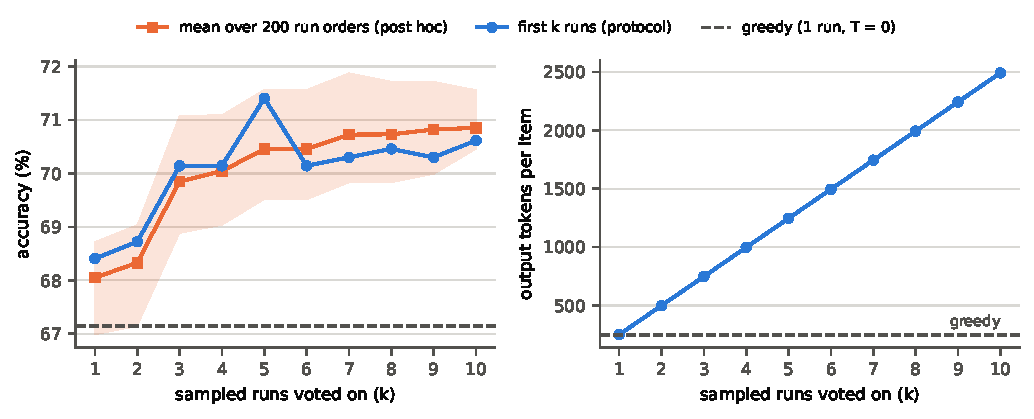
\includegraphics[width=0.86\textwidth]{figures/fig2b_majority_of_k_orders.pdf}
\Description{Two line charts. Left: accuracy of a majority over k sampled runs for k from 1 to 10, as the protocol's
first-k curve and as the mean over 200 random run orders with a shaded band, both above a dashed line for greedy
decoding. Right: output tokens per item growing linearly with k.}
\caption{Majority of $k$ sampled runs. Left: accuracy for the first $k$ runs (protocol) and averaged over 200 random
run orders with the 2.5--97.5 percentile band (post hoc); dashed line: greedy decoding. Right: output tokens per item.}
\label{fig:k}
\end{figure}

\subsection{RQ2 and RQ3: consistency and agreement}
Measured like for like, greedy decoding repeated its letter for \rerunSamePct\% of items, whereas two sampled runs at
$T$ = 0.7 agreed for \pairAgree\%; all ten agreed for only \unanimity\% (Table~\ref{tab:consistency}), with Fleiss'
$\kappa$ \kappaRuns. The distribution of modal shares was broadly similar for management and other items
(Figure~\ref{fig:agree}b).

The modal share separated correct from wrong votes with an AUROC of \auroc{} (95\% CI \aurocLo--\aurocHi), so H3 is
\emph{supported}. When at least 9 of 10 runs agreed (\nGeNine{} items) the vote was correct for \accGeNine\%, otherwise
(\nLtNine{} items) for \accLtNine\%; answering only unanimous items would cover \coverageTen\% of the test set at
\accTen\% accuracy (Figure~\ref{fig:agree}a). The signal needs many runs and partly reflects item difficulty (post hoc,
Table~\ref{tab:consistency}): with only the first 3 runs the AUROC was \aurocFirstThree, whether greedy agreed with the
vote gave \aurocGreedyAgree, and the 10-run modal share predicted the \emph{greedy} answer's correctness about as well
(\aurocGreedyCorrect). \unanimousWrong{} of the \unanimousN{} unanimous items (\unanimousWrongPct\%) were unanimously
wrong.

\paragraph{Shared answer-position preference (post hoc).} Keys were spread evenly over A--D, yet wrong answers rarely
chose A: \wrongAGreedy{} of \wrongGreedyN{} wrong greedy answers (\wrongAGreedyExp{} expected; $p$ = \wrongLettersP) and
\wrongASampled{} of \wrongSampledN{} wrong sampled answers (\wrongASampledExp{} expected). Accuracy was lowest when the key
was A (greedy \accGreedyKeyA\%, vote \accVoteKeyA\%, against \accGreedyKeyOtherMin--\accGreedyKeyOtherMax\% and
\accVoteKeyOtherMin--\accVoteKeyOtherMax\% otherwise). A preference shared by all runs correlates their errors, which
limits what a vote can correct; it may also reflect item content.

\begin{table}[t]
\caption{RQ2 and RQ3 for the 10 sampled runs at $T$ = 0.7 (\nTest{} items); percentile bootstrap CIs over items.}
\label{tab:consistency}
\footnotesize
\begin{tabular}{@{}lr@{}}
\toprule
Measure & Estimate (95\% CI) \\
\midrule
Unanimity, 10/10 runs (\%) & 49.4 (45.5, 53.2) \\
Mean modal share & 0.858 (0.843, 0.872) \\
Fleiss' $\kappa$ across runs & 0.715 (0.689, 0.738) \\
Pairwise flip rate (\%) & 21.4 (19.5, 23.3) \\
AUROC, modal share vs.\ vote correct & 0.737 (0.695, 0.780) \\
Vote accuracy, $\geq$9/10 agree ($n$ = 406) (\%) & 83.5 \\
Vote accuracy, $<$9/10 agree ($n$ = 227) (\%) & 47.6 \\
Coverage / accuracy at 10/10 agreement (\%) & 49.4 / 86.9 \\
\midrule
\multicolumn{2}{@{}l}{\emph{Post hoc comparisons}} \\
Pairwise agreement between two sampled runs (\%) & 78.6 \\
AUROC, modal share of first 3 runs vs.\ vote correct & 0.644 (0.604, 0.685) \\
AUROC, greedy agrees with vote vs.\ vote correct & 0.586 (0.551, 0.621) \\
AUROC, modal share vs.\ greedy correct & 0.749 (0.709, 0.788) \\
\bottomrule
\end{tabular}

\end{table}

\begin{figure}[t]
\centering
\begin{minipage}[b]{0.36\textwidth}\centering
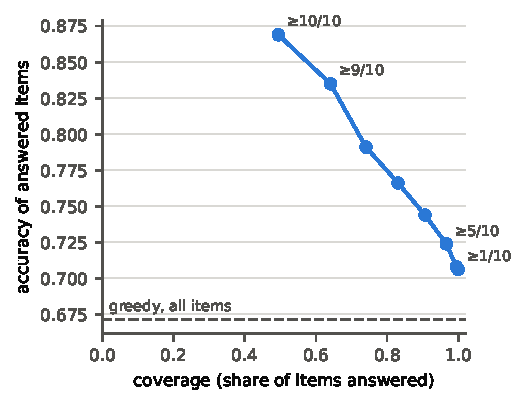
\includegraphics[width=\linewidth]{figures/fig3_accuracy_coverage.pdf}\\(a)
\end{minipage}\hfill
\begin{minipage}[b]{0.45\textwidth}\centering
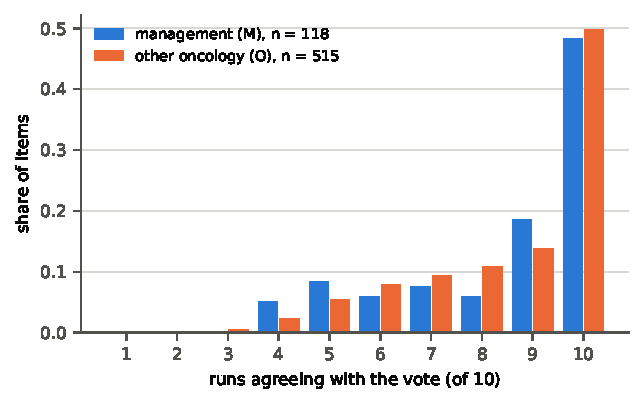
\includegraphics[width=\linewidth]{figures/fig4_modal_share.pdf}\\(b)
\end{minipage}
\Description{(a) A line chart of accuracy against coverage: accuracy rises as fewer items are answered, from the
full test set to items with all 10 runs agreeing, all above a dashed line for greedy decoding. (b) A bar chart of the
share of items by number of runs agreeing with the vote, for management and other items; the largest bars are at 10.}
\caption{(a) Accuracy against coverage when only items with at least $x$ of 10 agreeing runs are answered (dashed:
greedy on all items). (b) Runs agreeing with the vote, for management (M) and other oncology (O) items.}
\label{fig:agree}
\end{figure}

\subsection{Exploratory analyses (protocol amendment)}
A second greedy run of all items scored \accRerun\%, \rerunDiff{} points from the first (\rerunDiffLo{} to
\rerunDiffHi). At $T$ = 0.3 the vote reached \accVoteTLow\% and gained \diffTLow{} points over greedy; its bootstrap
interval (\diffTLowLo{} to \diffTLowHi) excludes zero but the McNemar test does not ($p$ = \pTLow), so it would not
meet the frozen rule, which requires both. At $T$ = 1.0 the vote reached \accVoteTHigh\%, a gain of \diffTHigh{} points
(\diffTHighLo{} to \diffTHighHi; $p$ = \pTHigh). Unanimity was \unanimityTLow\%, \unanimity\% and \unanimityTHigh\% at
$T$ = 0.3, 0.7 and 1.0; in a post hoc paired comparison it was lower at 1.0 than at 0.3 by \unanDiffHighLow{} points
(\unanDiffHighLowLo{} to \unanDiffHighLowHi), while 0.7 and 1.0 did not differ clearly (\unanDiffHighMidLo{} to
\unanDiffHighMidHi). The AUROC stayed between \aurocTLow{} and \aurocTHigh. The contamination probe reproduced the hidden
option exactly for \probeHits{} of \probeN{} items (Wilson interval \probeLo--\probeHi\%), \probeShortHits{} of them
among the \probeShortN{} options of one or two words, which can be guessed.

\subsection{Error analysis}
By construction, on the \bMain{} items where only the vote was right greedy's letter was not the majority letter; the
informative part is how rare it was: it appeared in \bGreedyLetterRunsParsed{} of the 10 sampled runs on average (for
the \bParsedN{} items with a parsed greedy answer), while the correct letter appeared in \bKeyRuns. On the \cMain{}
items where only greedy was right, the correct letter appeared in \cKeyRuns{} of 10 runs. \tiesB{} and \tiesC{} of
these items, respectively, were decided by the tie rule. \allWrong{} items were answered wrongly in all 11
generations: in \allWrongSame{} every generation chose the same wrong option (these are exactly the unanimously wrong
items), \allWrongMixed{} had two or more different wrong options, and \allWrongUnparseable{} mixed a wrong option with
unparseable output.

As an anecdotal check, the AI assistant read two random items per category: greedy sometimes named the right
finding but chose another option; runs sometimes split between two plausible options; in one item several runs
declined to choose; and in always-wrong items every run reasoned towards a non-keyed diagnosis or mechanism. No
clinician checked these readings.
